\documentclass[12pt]{article}

\usepackage[utf8x]{inputenc} % Включаем поддержку UTF8  
\usepackage[russian]{babel}  % Включаем пакет для поддержки русского языка  
\usepackage{hyperref}        % Для гиперссылок

% Математика
\usepackage{amsmath,amsfonts,amssymb,amsthm,mathtools} % AMS
\usepackage{icomma}
\usepackage{mathrsfs}

\usepackage{xcolor}

% Прога
\usepackage{etoolbox}
\usepackage{listings}

\definecolor{codegreen}{rgb}{0,0.6,0}
\definecolor{codegray}{rgb}{0.5,0.5,0.5}
\definecolor{codepurple}{rgb}{0.58,0,0.82}
\definecolor{backcolour}{rgb}{0.95,0.95,0.92}

\lstdefinestyle{mystyle}{
	backgroundcolor=\color{backcolour},   
	commentstyle=\color{codegreen},
	keywordstyle=\color{magenta},
	numberstyle=\tiny\color{codegray},
	stringstyle=\color{codepurple},
	basicstyle=\ttfamily\footnotesize,
	breakatwhitespace=false,         
	breaklines=true,                 
	captionpos=b,                    
	keepspaces=true,                 
	numbers=left,                    
	numbersep=5pt,                  
	showspaces=false,                
	showstringspaces=false,
	showtabs=false,                  
	tabsize=2
}

\lstset{style=mystyle}

% Цвета
\usepackage{xcolor}

% Картинки
\usepackage{graphicx}
\graphicspath{ {./images/} }

\usepackage{tikzsymbols}

% Работа с таблицами
\usepackage{array,tabularx,tabulary,booktabs} % Дополнительная работа с таблицами
\usepackage{longtable}  % Длинные таблицы
\usepackage{multirow} % Слияние строк в таблице

% Нумерованные списки
\usepackage[shortlabels]{enumitem} % Разные лейблы

% Текст
\usepackage[normalem]{ulem}  % для зачеркивания текста

\newtheorem{property}{Свойство}
\newtheorem{consequence}{Следствие}[property]

\DeclarePairedDelimiter\abs{\lvert}{\rvert}%
\DeclarePairedDelimiter\norm{\lVert}{\rVert}%

% Swap the definition of \abs* and \norm*, so that \abs
% and \norm resizes the size of the brackets, and the 
% starred version does not.
\makeatletter
\let\oldabs\abs
\def\abs{\@ifstar{\oldabs}{\oldabs*}}
%
\let\oldnorm\norm
\def\norm{\@ifstar{\oldnorm}{\oldnorm*}}
\makeatother

\begin{document}
	
	\thispagestyle{empty}
	\begin{center}
		\textbf{ПРАВИТЕЛЬСТВО РОССИЙСКОЙ ФЕДЕРАЦИИ}
		
		\vspace{5ex}
		
		\textbf{Федеральное государственное автономное образовательное учреждение \\ высшего образования \\ <<Национальный исследовательский университет \\ <<Высшая школа экономики>>}
	\end{center}
	\vspace{5ex}
	
	\begin{center}
		Московский институт электроники и математики им. А.Н. Тихонова  
		
		\vspace{5ex}
		
		Департамент прикладной математики
		
		\vspace{10ex}
		\textbf{Отчёт \\ по лабораторной работе №11 \\ по курсу <<Алгоритмизация и программирование>> \\ Задание № 13}
		\vspace{7ex}
		
	\end{center}
	
	\begin{center} 
		\begin{tabular}{| p{0.3\linewidth}| p{0.3\linewidth}| p{0.3\linewidth}|}
			\hline	
			ФИО студента & Номер группы & Дата \\  \hline
			& & \\  
			Кейер Александр \newline Петрович & БПМ-231 & \today\\  
			& & \\  \hline		
		\end{tabular}
	\end{center}
	
	\begin{center}
		\vspace{3ex}
		
		\vfill
		
		\normalsize
		
		\textbf{Москва, 2023}
	\end{center}
	
	\newpage
	
	%---------------------------------------------------------------------------------
	
	\section{Задание (вариант № 13)}
	
	
	
\includegraphics[width=\linewidth]{images/task}

	
	\newpage
	
	\section{Структура заголовочного файла}
	
	\begin{lstlisting}[language=C]
		struct Footballer {
			char* fullName;
			char* clubName;
			char* role;
			int age;
			int numberOfGames;
			int numberOfGoals;
		};
		
		typedef struct Footballer Footballer;
	\end{lstlisting}
	
	\section{Решение}
	
	\begin{lstlisting}[language=C]
		#include <stdio.h> // Input/output library.
		#include <stdlib.h> // Memory allocation.
		#include <time.h> // Time library.
		#include <assert.h> // Assertion library.
		#include <string.h> // String functions library.
		
		#include "football.h" // Footballer info.
		
		#define TIME 1000000000
		
		// Function printing horizontal line.
		void printHr(int length) {
			for (int j = 0; j < length; j++) {
				printf("- ");
			}
			printf("\n");
		}
		
		// Function printing table header.
		void printTableHeader() {
			printHr(65);
			printf("%4s|%30s|%30s|%30s|%10s|%10s|%10s|\n", "ID", "FULL NAME", "CLUB NAME", "ROLE", "AGE", "GAMES", "GOALS");
			printHr(65);
		}
		
		// Function printing footballer.
		void printFootballer(Footballer* footballer) {
			printf("%4s|%30s|%30s|%30s|%10d|%10d|%10d|\n", "?", footballer->fullName, footballer->clubName, footballer->role, footballer->age, footballer->numberOfGames, footballer->numberOfGoals);
			printHr(65);
		}
		
		// Function printing footballers.
		void printFootballersArray(Footballer* footballers, int length) {
			if (footballers == NULL) {
				printf("Incorrect array.\n");
				return;
			}
			
			printTableHeader();
			
			for (int i = 0; i < length; i++) {
				printFootballer(footballers + i);
			}
		}
		
		// Function generating string.
		char* generateString(int length, int countOfUsedSymbols) {
			assert(countOfUsedSymbols <= 26);
			
			char* out = (char*)malloc(sizeof(char) * (length + 1));
			char alphabet[26] = {
				'a', 'b', 'c', 'd', 'e', 'f', 'g', 'h', 'i', 'j', 'k', 'l', 'm',
				'n', 'o', 'p', 'q', 'r', 's', 't', 'u', 'v', 'w', 'x', 'y', 'z'
			};
			
			for (int i = 0; i < length; i++) {
				out[i] = alphabet[rand() % countOfUsedSymbols];
			}
			
			out[length] = '\0';
			
			return out;
		}
		
		// Function generating footballer.
		Footballer generateFootballer(int rand1, int rand2) {
			Footballer out = {
				.fullName=generateString(rand1 % 26, rand2 % 26),
				.clubName=generateString(10, 26),
				.role=generateString(10, 26),
				.age=(rand() % 100),
				.numberOfGames=(rand() % 100),
				.numberOfGoals=(rand() % 100),
			};
			
			return out;
		}
		
		// Function generating footballer array.
		Footballer* generateFootballersArray(int length, int rand1, int rand2) {
			Footballer* arr = (Footballer*)malloc(sizeof(Footballer) * length);
			
			for (int i = 0; i < length; i++) {
				arr[i] = generateFootballer(rand1, rand2);
			}
			
			// printf("Successfully generated %d footballers array.\n", length);
			return arr;
		}
		
		// Function comparing footballers.
		int compareFootballers(Footballer* footballer1, Footballer* footballer2, int direction) {
			return strcmp(footballer1->fullName, footballer2->fullName);
		}
		
		struct Node {
			Footballer* footballer;
			struct Node* left;
			struct Node* right;
		};
		typedef struct Node Node;
		
		Node* createNode(Footballer* footballer) {
			Node* node = (Node*)malloc(sizeof(Node));
			
			node->footballer = footballer;
			node->left = node->right = NULL;
			
			return node;
		}
		
		Node* insertNode(Node* root, Node* insertionNode) {
			if (root == NULL) {
				return insertionNode;
			}
			
			if (compareFootballers(insertionNode->footballer, root->footballer, 1) >= 0) {
				root->right = insertNode(root->right, insertionNode);
			} else {
				root->left = insertNode(root->left, insertionNode);
			}
			
			return root;
		}
		
		void insertNodeByFootballer(Node* root, Footballer* footballer) {
			insertNode(root, createNode(footballer));
		}
		
		Node* createTreeFromFootballersArray(Footballer* footballers, int footballersCount) {
			Node* root = createNode(&footballers[0]);
			
			for (int i = 1; i < footballersCount; i++) {
				insertNodeByFootballer(root, footballers + i);
			}
			
			return root;
		}
		
		void printFootabllersBinarySearchTree(Node* root) {
			if (root == NULL) {
				return;
			}
			
			printFootabllersBinarySearchTree(root->left);
			printFootballer(root->footballer);
			printFootabllersBinarySearchTree(root->right);
		}
		
		void printNodesArray(Node** nodes, int nodesCount) {
			if (nodesCount == 0) {
				printf("Footballers with this name were not found.\n");
			}
			
			for (int i = 0; i < nodesCount; i++) {
				printFootballer(nodes[i]->footballer);
			};
		}
		
		Node* findNodeInBinarySearchTreeByFootballerFullName(Node* root, char* fullName) {
			if (root == NULL || strcmp(root->footballer->fullName, fullName) == 0) {
				return root;
			}
			
			if (strcmp(root->footballer->fullName, fullName) > 0) {
				return findNodeInBinarySearchTreeByFootballerFullName(root->left, fullName);
			}
			
			return findNodeInBinarySearchTreeByFootballerFullName(root->right, fullName);
		}
		
		int findAllNodesInBinarySearchTreeByFootballerFullName(Node* root, char* fullName, Node** nodes) {
			Node* curNode = findNodeInBinarySearchTreeByFootballerFullName(root, fullName);
			
			int nodesCount = 0;
			
			if (curNode == NULL) {
				nodes = NULL;
				
				return nodesCount;
			}
			
			nodes[0] = curNode;
			nodesCount++;
			
			Node* nextNode = curNode->right;
			
			while (nextNode != NULL && strcmp(curNode->footballer->fullName, nextNode->footballer->fullName) == 0) {
				nodes[nodesCount] = nextNode;
				nextNode = nextNode->right;
				nodesCount++;
			}
			
			return nodesCount;
		}
		
		// =================
		// Hash table dope.
		// Hash table crazy.
		// Hash table here.
		// =================
		
		struct ListItem {
			Footballer* footballer;
			struct ListItem* next;
		};
		typedef struct ListItem ListItem;
		
		ListItem* createListItem(Footballer* footballer) {
			ListItem* listItem = (ListItem*)malloc(sizeof(ListItem));
			
			listItem->footballer = footballer;
			listItem->next = NULL;
			
			return listItem;
		}
		
		struct HashTable {
			int size;
			ListItem** table;
		};
		typedef struct HashTable HashTable;
		
		HashTable* createHashTable(int size) {
			HashTable* hashTable = (HashTable*)malloc(sizeof(HashTable));
			ListItem** table = (ListItem**)malloc(sizeof(ListItem*) * size);
			
			hashTable->table = table;
			hashTable->size = size;
			
			for (int i = 0; i < size; i++) {
				table[i] = NULL;
			}
			
			return hashTable;
		}
		
		int hashFunction(HashTable* hashTable, char* fullName) {
			int hash = 0;
			
			while (*fullName != 0) {
				hash = (hash + *fullName++) % hashTable->size;
			}
			
			return hash;
		}
		
		void insertFootballerIntoHashTable(HashTable* hashTable, Footballer* footballer) {
			int hash = hashFunction(hashTable, footballer->fullName);
			
			ListItem* listItem = createListItem(footballer);
			
			listItem->next = hashTable->table[hash];
			hashTable->table[hash] = listItem;
		}
		
		HashTable* createHashTableFromFootballersArray(Footballer* footballers, int footballersCount) {
			HashTable* hashTable = createHashTable(footballersCount);
			
			for (int i = 0; i < footballersCount; i++) {
				insertFootballerIntoHashTable(hashTable, footballers + i);
			}
			
			return hashTable;
		}
		
		int findAllListItemsInHashTableByFootballerFullName(HashTable* hashTable, char* fullName, ListItem** listItems) {
			int hash = hashFunction(hashTable, fullName);
			
			int listItemsCount = 0;
			
			ListItem* listItem = hashTable->table[hash];
			
			while (listItem != NULL) {
				if (strcmp(listItem->footballer->fullName, fullName) == 0) {
					listItems[listItemsCount] = listItem;
					listItemsCount++;
				}
				
				listItem = listItem->next;
			}
			
			return listItemsCount;
		}
		
		void printFootballersHashTable(HashTable* hashTable) {
			for (int hash = 0; hash < hashTable->size; hash++) {
				if (hashTable->table[hash] == NULL) {
					continue;
				}
				
				ListItem* listItem = hashTable->table[hash];
				
				while (listItem != NULL) {
					printFootballer(listItem->footballer);
					
					listItem = listItem->next;
				}
			}
		}
		
		void printFootballersListItems(ListItem** listItems, int listItemsCount) {
			if (listItemsCount == 0) {
				printf("Footballers with this name were not found.\n");
				return;
			}
			
			for (int i = 0; i < listItemsCount; i++) {
				printFootballer(listItems[i]->footballer);
			}
		}
		
		// Function to free memory allocated for binary search tree nodes.
		void freeBinarySearchTreeNodes(Node* root) {
			if (root == NULL) {
				return;
			}
			
			freeBinarySearchTreeNodes(root->left);
			freeBinarySearchTreeNodes(root->right);
			
			// Free the node itself.
			free(root);
		}
		
		// Function to free memory allocated for hash table list items.
		void freeHashTableListItems(HashTable* hashTable) {
			for (int i = 0; i < hashTable->size; i++) {
				ListItem* listItem = hashTable->table[i];
				
				while (listItem != NULL) {
					ListItem* temp = listItem;
					listItem = listItem->next;
					
					// Free the list item itself.
					free(temp);
				}
			}
		}
		
		int testsCounter = 1;
		
		void test(int footballersCount, char* fullName, int rand1, int rand2, int* binaryTreeAccTime, int* hashTableAccTime, int printEveryTest) {
			if (printEveryTest) {
				printf("\n============================================================= Test %d =============================================================\n\n", testsCounter++);
				printf("Name=\"%s\"\n", fullName);
			}
			
			// Prepare program and generate footballers array.
			
			Footballer* footballers = generateFootballersArray(footballersCount, rand1, rand2);
			
			// printf("\nPrint footballers array.\n");
			// printFootballersArray(footballers, footballersCount);
			
			// printf("\n==== Binary tree ====\n");
			
			// Create binary search tree.
			
			Node* root = createTreeFromFootballersArray(footballers, footballersCount);
			
			// printf("\nPrint footballers binary tree.\n");
			// printTableHeader();
			// printFootabllersBinarySearchTree(root);
			
			// Work with binary search tree.
			
			Node** nodes = (Node**)malloc(sizeof(Node*) * footballersCount);
			
			clock_t start = clock();
			
			int nodesCount = findAllNodesInBinarySearchTreeByFootballerFullName(root, fullName, nodes);
			
			clock_t stop = clock();
			
			if (printEveryTest) {
				printf("BinarySearchTree %4s%7d: %.00fns\n", "n=", footballersCount, (double)(stop - start) / CLOCKS_PER_SEC * TIME);
			}
			
			*binaryTreeAccTime += (double)(stop - start) / CLOCKS_PER_SEC * TIME;
			
			// printf("\nAll nodes with footballer fullName = \"%s\".\n", fullName);
			// printTableHeader();
			// printNodesArray(nodes, nodesCount);
			
			// printf("\n==== Hash table ====\n");
			
			// Create hash table.
			
			HashTable* hashTable = createHashTableFromFootballersArray(footballers, footballersCount);
			
			// printf("\nPrint footballers hash table.\n");
			// printTableHeader();
			// printFootballersHashTable(hashTable);
			
			// Work with hash table.
			
			ListItem** listItems = (ListItem**)malloc(sizeof(ListItem*) * footballersCount);
			
			start = clock();
			
			int listItemsCount = findAllListItemsInHashTableByFootballerFullName(hashTable, fullName, listItems);
			
			stop = clock();
			
			if (printEveryTest) {
				printf("HashTable %11s%7d: %.00fns\n", "n=", footballersCount, (double)(stop - start) / CLOCKS_PER_SEC * TIME);
			}
			
			*hashTableAccTime += (double)(stop - start) / CLOCKS_PER_SEC * TIME;
			
			// printf("\nAll list items with footballer fullName = \"%s\".\n", fullName);
			// printTableHeader();
			// printFootballersListItems(listItems, listItemsCount);
			
			// End program and free allocated memory.
			
			freeBinarySearchTreeNodes(root);
			freeHashTableListItems(hashTable);
			
			free(nodes);
			free(listItems);
			
			// Free the memory allocated for the footballers array and the strings inside it.
			for (int i = 0; i < footballersCount; i++) {
				free(footballers[i].fullName);
				free(footballers[i].clubName);
				free(footballers[i].role);
			}
			
			free(footballers);
		}
		
		void runTests(int footballersCount, int testsCount, int printEveryTest) {
			srand(time(NULL)); // Init first random number.
			
			int rand1 = rand() % 26;
			int rand2 = rand() % 26;
			
			int binaryTreeAccTime = 0;
			int hashTableAccTime = 0;
			
			for (int i = 0; i < testsCount; i++) {
				test(footballersCount, generateString(rand1, rand2), rand1, rand2, &binaryTreeAccTime, &hashTableAccTime, printEveryTest);
			}
			
			printf("\n============================================================= Average from %d tests =============================================================\n\n", testsCount);
			
			printf("BinarySearchTree %4s%7d: %.00fns\n", "footballersCount=", footballersCount, (double)(binaryTreeAccTime / testsCount));
			printf("HashTable %24s%7d: %.00fns\n", "footballersCount=", footballersCount, (double)(hashTableAccTime / testsCount));
			
			printf("\n\n");
		}
		
		int main() {
			printf("Lab 11. Keyer, BAM231.\n");
			
			runTests(1000, 100, 0);
			runTests(5000, 100, 0);
			runTests(10000, 100, 0);
			runTests(20000, 100, 0);
			runTests(50000, 100, 0);
			runTests(100000, 100, 0);
			runTests(1000000, 100, 0);
			
			return 0;
		}

	\end{lstlisting}

	
	\section{Тесты}
	
	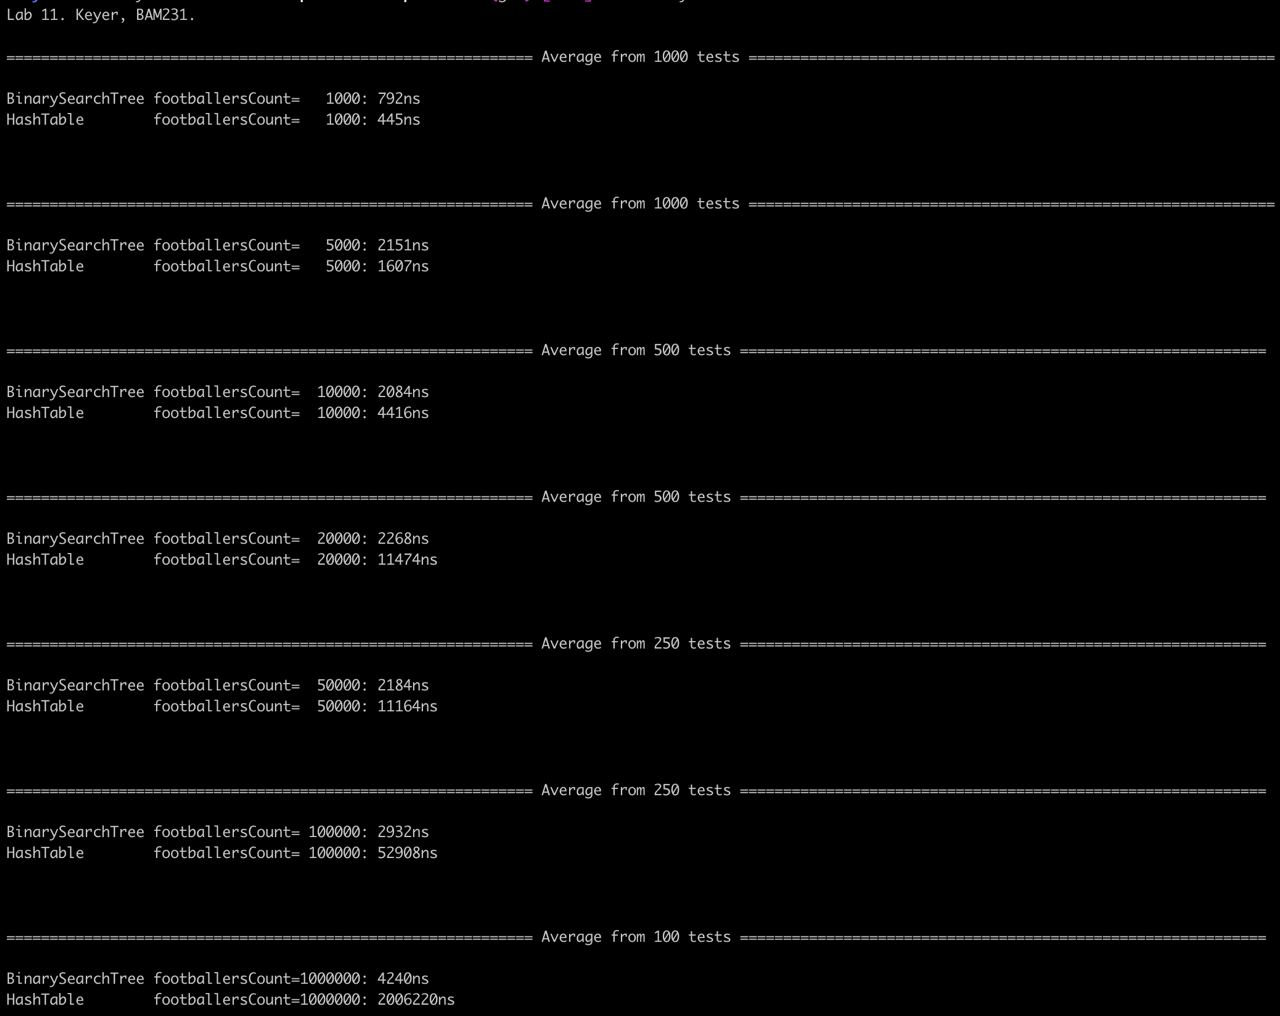
\includegraphics[width=2\linewidth]{images/tests}
	
	Для каждого количества футболистов было проведено свое количество тестов и взято среднее арифметическое в наносекундах, потраченных на поиск всех футболистов с определенным именем.
	\begin{enumerate}
		\item Имена в каждом тести генерировались автоматически: максимальное количество букв в имени 26, использовать можно было тоже только 26 латинских букв. Суммарно тесты покрывают каждую возможную длину имени и разное количество букв, из которых оно состоит
		\item Забавно, но это замеры на Mac M3. Если взять Intel и Windows 11, но все тот же GCC, то там поиск по бинарному дереву всегда 0 наносекунд, а вот поиск по хеш-таблице оставляет желать лучшего.
	\end{enumerate}
	
	\section{Графики}


	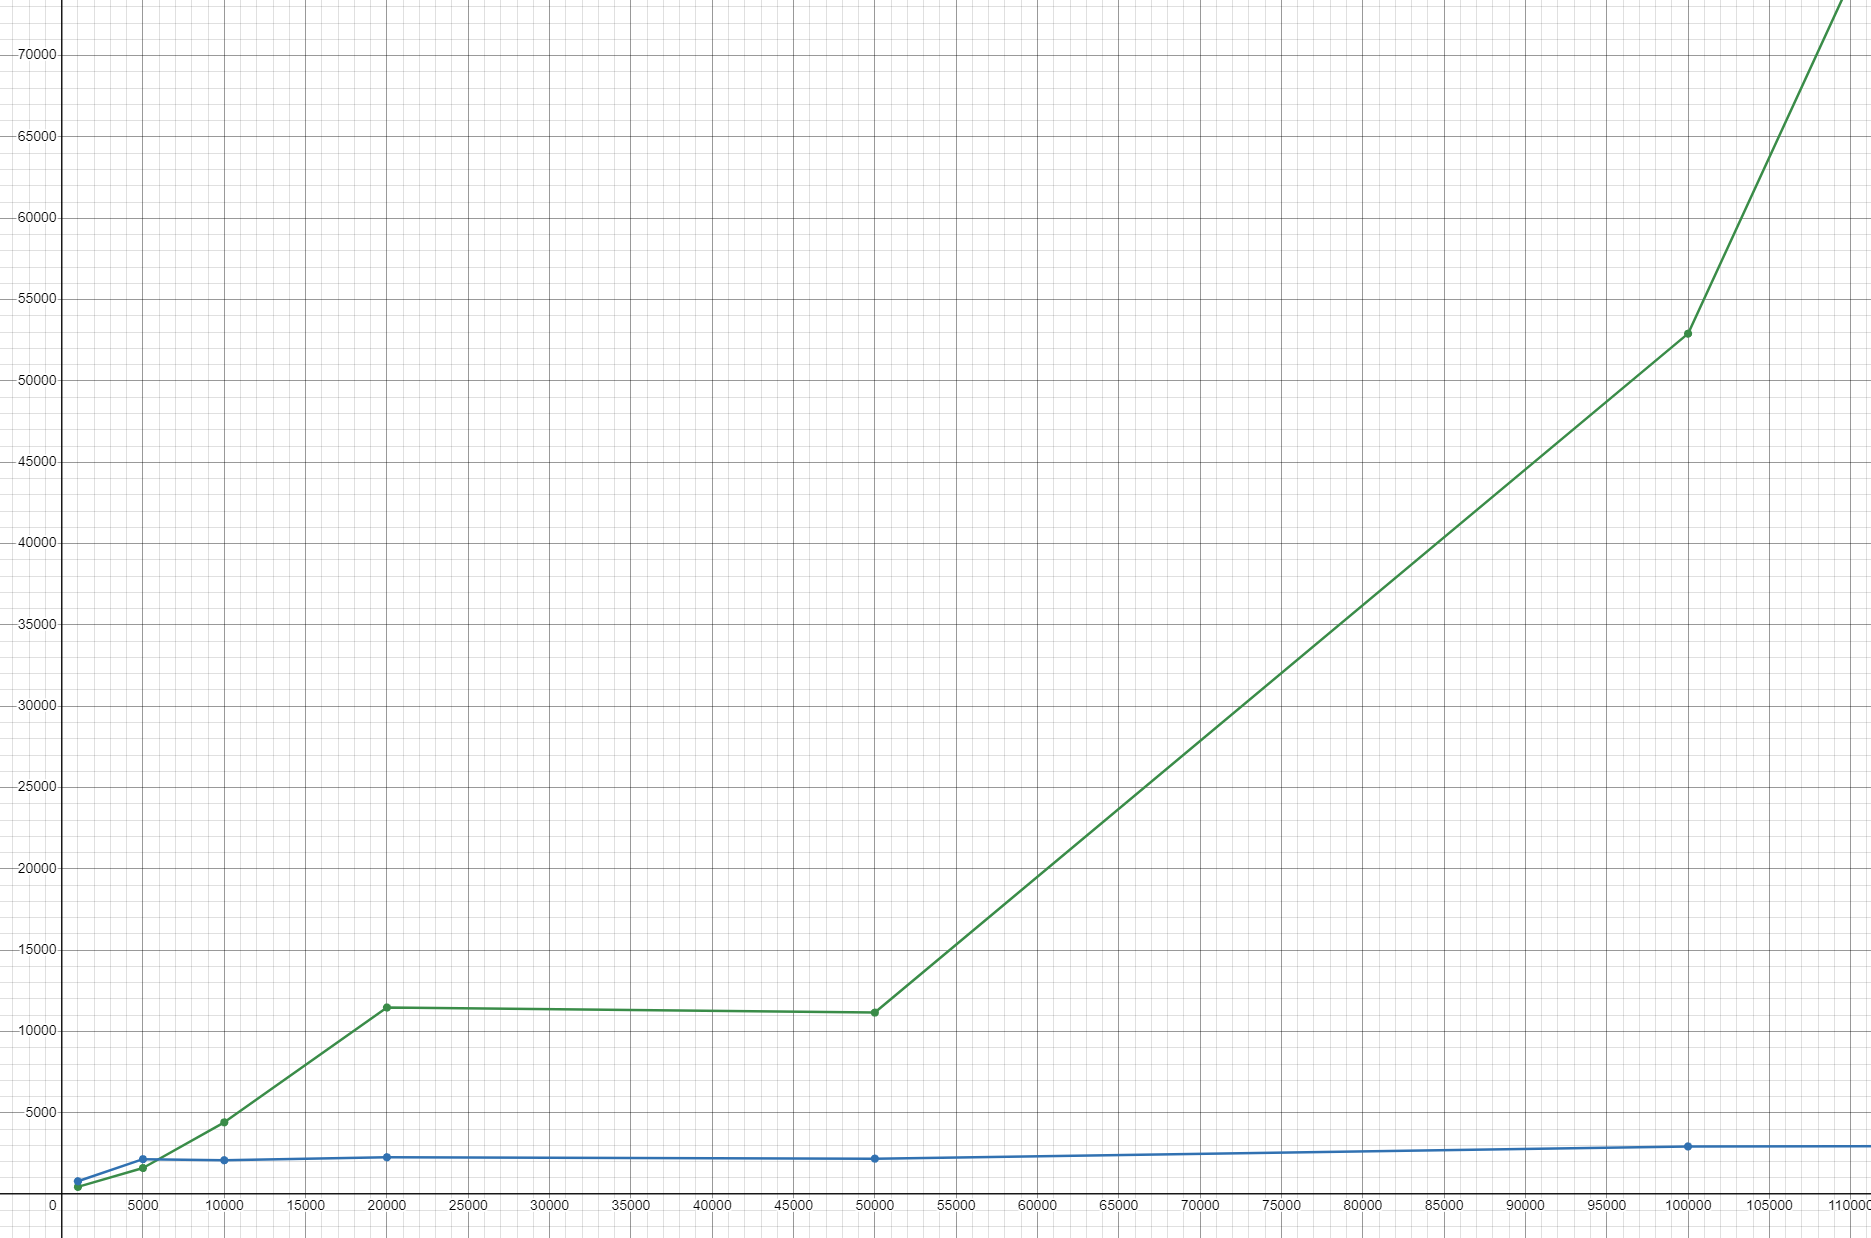
\includegraphics[width=\linewidth]{images/graphics_1}
	
	У бинарного дерево, как и должно быть, идет нечто похожее на логарифм, а у хеш-таблицы на обычную линейную функцию.
	
	

	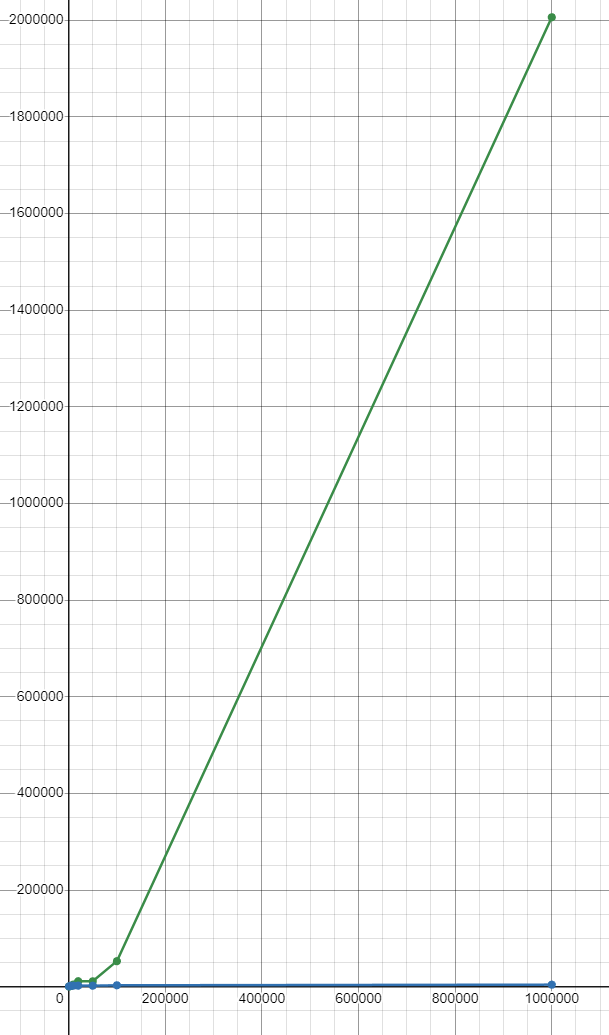
\includegraphics[width=\linewidth]{images/graphics}
	
\end{document}
